\documentclass{article}
\usepackage{ctex}
\usepackage{blindtext}
\usepackage[utf8]{inputenc}
\usepackage{amsmath,bm}
\usepackage{amstext}
\usepackage{amsfonts}
\usepackage{amsmath}
%行间距
\usepackage{setspace}
%图片
\usepackage{subfigure}         
\usepackage{natbib}
\usepackage{float}
\usepackage{epstopdf}
\usepackage{graphicx}

\title{Introduction to Machine Learning\\Homework 1}
\begin{document}
	\maketitle
	\numberwithin{equation}{section}
	%\newpage
	
	\section{[20pts] Basic review of probability}
	The probability distribution of random variable $X$ follows:\\
	\begin{equation}
	f_X(x)=\begin{cases}
	\frac{1}{2} & 0<x<1;\\
	\frac{1}{6} & 2<x<5;\\
	0 & \text{otherwise}.
	\end{cases}
	\end{equation} 
	(1) [5pts] Please give the cumulative distribution function $F_X(x)$ for X;\\ \\ 
	(2) [5pts] Define random variable $Y$ as $Y=1/(X^2)$, please give the probability density function $f_Y(y)$ for $Y$;\\ \\
	(3) [10pts] For some random non-negative random variable Z, please prove the following two formulations are equivalent:\\
	\begin{equation}
	\mathbb{E}[Z]=\int^\infty_{z=0} z f(z)\mathrm{d}z,
	\end{equation}
	\begin{equation}
	\mathbb{E}[Z]=\int^\infty_{z=0} \mathrm{Pr}[Z\geq z]\mathrm{d}z,
	\end{equation}
	Meantime, please calculate the expectation of random variable $X$ and $Y$ by these two expectation formulations to verify your proof.
	\newpage
	\begin{spacing}{2.0}
	\textbf{解:}
	(1)
	$x\leq 0$, 
	$F_X(x)=\int_{-\infty}^{x}f_X(x)\mathrm{d}x
	=\int_{-\infty}^{x}0\mathrm{d}x=0$\\
	$0<x<1$, 
	$F_X(x)=\int_{-\infty}^{x}f_X(x)\mathrm{d}x
	=\int_{-\infty}^{0}0\mathrm{d}x+\int_{0}^{x}\frac{1}{2}\mathrm{d}x
	=\frac{x}{2}$\\
	$1\leq x\leq 2$,
	$F_X(x)=\int_{-\infty}^{x}f_X(x)\mathrm{d}x
	=\int_{-\infty}^{0}0\mathrm{d}x+\int_{0}^{1}\frac{1}{2}\mathrm{d}x+\int_{1}^{x}0\mathrm{d}x
	=\frac{1}{2}$\\
	$2<x<5$, 
	$F_X(x)=\int_{-\infty}^{0}0\mathrm{d}x
	+\int_{0}^{1}\frac{1}{2}\mathrm{d}x
	+\int_{1}^{2}0\mathrm{d}x
	+\int_{2}^{x}\frac{1}{6}\mathrm{d}x
	=\frac{1}{6}x+\frac{1}{6}$\\
	$x\geq 5$,
	$F_X(x)=\int_{-\infty}^{0}0\mathrm{d}x
	+\int_{0}^{1}\frac{1}{2}\mathrm{d}x
	+\int_{1}^{2}0\mathrm{d}x
	+\int_{2}^{5}\frac{1}{6}\mathrm{d}x
	+\int_{5}^{x}0\mathrm{d}x
	=1$\\
	\begin{spacing}{1.0}
	\begin{equation}
		F_X(x)=\begin{cases}
		0 & x\leq 0\\
		\frac{x}{2} & 0<x<1\\
		\frac{1}{2} & 1\leq x\leq 2\\
		\frac{1}{6}x+\frac{1}{6} & 2<x<5\\
		1 & x\geq 5
		\end{cases}
	\end{equation}\\
	\end{spacing}

	(2)
	$F_Y(y)=P(Y\leq y)
	=P(\frac{1}{X^2}\leq y)
	=P(X\geq \frac{1}{\sqrt{y}})$\\
	$y\leq 0$, $F_Y(y)=0$\\
	$\frac{1}{\sqrt{y}}\geq 5$, $0<y\leq \frac{1}{25}$,
	$F_Y(y)=0$\\
	$2<\frac{1}{\sqrt{y}}< 5$, $\frac{1}{25}<y<\frac{1}{4}$,
	$F_Y(y)
	=\int_{\frac{1}{\sqrt{y}}}^{5}\frac{1}{6}\mathrm{d}x
	=\frac{5}{6}-\frac{1}{6\sqrt{y}}$\\
	$1\leq \frac{1}{\sqrt{y}}\leq 2$, $\frac{1}{4}\leq y\leq 1$,
	$F_Y(y)
	=\int_{2}^{5}\frac{1}{6}\mathrm{d}x
	=\frac{1}{2}$\\
	$0<\frac{1}{\sqrt{y}}< 1$, $y>1$,
	$F_Y(y)
	=\int_{2}^{5}\frac{1}{6}\mathrm{d}x+\int_{\frac{1}{\sqrt{y}}}^{1}\frac{1}{2}\mathrm{d}x
	=1-\frac{1}{2\sqrt{y}}$\\
	\begin{spacing}{1.0}
		\begin{equation}
			f_Y(y)=F_Y'(y)=\begin{cases}
			\frac{1}{12y\sqrt{y}} & \frac{1}{25}<y<\frac{1}{4}\\
			\frac{1}{4y\sqrt{y}} & y>1\\
			0 & \text{otherwise}
			\end{cases}
		\end{equation}\\
	\end{spacing}

	(3)
	$\mathbb{E}[Z]
	=\int_{z=0}^\infty \mathrm{Pr}[Z\geq z]\mathrm{d}z
	=\int_{z=0}^\infty [\int_{x}^\infty f(t)\mathrm{d}t]\mathrm{d}z
	=\int_{0}^{\infty}[\int_{0}^{t}f(t)\mathrm{d}z]\mathrm{d}t
	=\int_{0}^{\infty}tf(t)\mathrm{d}t
	=\int_{z=0}^{\infty}zf(z)\mathrm{d}z$\\
	$\mathbb{E}[X]=\int_{0}^{\infty}xf_X(x)\mathrm{d}x
	=\int_{0}^{1}\frac{x}{2}\mathrm{d}x+\int_{2}^{5}\frac{x}{6}\mathrm{d}x
	=\frac{x^2}{4}|_0^1+\frac{x^2}{12}|_2^5
	=2$\\
	$\mathbb{E}[X]=\int_{0}^\infty \mathrm{Pr}[X\geq x]\mathrm{d}x
	=\int_{2}^{5}\frac{5-x}{6}\mathrm{d}x
	+\int_{1}^{2}\frac{1}{6}(5-2)\mathrm{d}x
	+\int_{0}^{1}(\frac{1-x}{2}+\frac{1}{2})\mathrm{d}x
	=(\frac{5}{6}x-\frac{x^2}{12})|_2^5+\frac{x}{2}|_1^2+(x-\frac{x^2}{4})|_0^1
	=2$\\
	$\mathbb{E}[Y]
	=\int_{0}^{\infty}yf(y)\mathrm{d}y
	=\int_{0}^{1}\frac{1}{x^2}\cdot\frac{1}{2}\mathrm{d}x
	+\int_{2}^{5}\frac{1}{x^2}\cdot\frac{1}{6}\mathrm{d}x
	=(-\frac{1}{2x})|_0^1+(-\frac{1}{6x})|_2^5$\\
	因此,两个公式计算出的$X$的数学期望相等,而$Y$的数学期望不存在。
	\end{spacing}





	\section{[15pts] Probability Transition}
	
	(1) [5pts] Suppose P(rain today) = 0.30, P(rain tomorrow) = 0.60,
	P(rain today and tomorrow) = 0.25. Given that it rains today, what
	is the probability it will rain tomorrow?\\\\
	(2) [5pts] Give a formula for $P(G | \neg H)$ in terms of $P(G)$,
	$P(H)$ and $P(G \wedge H)$ only.  Here $H$ and $G$ are boolean random variables.\\ \\
	(3) [5pts] A box contains {\it w} white balls and {\it b} black
	balls. A ball is chosen at random. The ball is then replaced,
	along with {\it d} more balls of the same color (as the chosen
	ball). Then another ball is drawn at random from the box. Show
	that the probability that the second ball is white does not depend
	on {\it d}.  
	
	\begin{spacing}{2.0}
	\textbf{解:}
	(1)
	$P(\text{rain tomorrow|rain today})
	=\frac{P(\text{rain today and tomorrow})}{P(\text{rain today})}
	=\frac{5}{6}$

	(2)
	$P(G|\neg H)=\frac{P(G\wedge\neg H)}{P(\neg H)}
	=\frac{P(G)-P(G\wedge H)}{1-P(H)}$

	(3)设$A_1$为第一次取到白球,$A_2$为第一次取到黑球,$B$为第二次取到白球。

	$P(B)=P(B|A_1)+P(B|A_2)
	=\frac{w}{w+b}*\frac{w+d}{w+b+d}+\frac{b}{w+b}*\frac{w}{w+b+d}
	=\frac{w}{w+b}$

	因此第二次取到白球的概率与$d$无关。
	\end{spacing}





	\section{[20pts] Basic review of Linear Algebra}
	Let $x = (\sqrt{3}, 1)^{\top}$ and $y = (1, \sqrt{3})^{\top}$ be two vectors,\\\\
	(1) [5pts] What is the value of $x_{\perp}$ where $x_{\perp}$ indicates the projection of $x$ onto $y$. \\\\
	(2) [5pts] Prove that $y \perp (x - x_{\perp})$.\\\\
	(3) [10pts] Prove that for any $\lambda \in \mathbb{R}$, $\lvert| x - x_{\perp}\rvert| \leq \lvert| x - \lambda y \rvert|$ 
	
	\begin{spacing}{2.0}
	\textbf{解:}
	(1)
	$x_{\perp}=(\frac{\sqrt{3}}{2},\frac{3}{2})^{\top}$

	(2)
	$x-x_{\perp}=(\sqrt{3}, 1)^{\top}-(\frac{\sqrt{3}}{2},\frac{3}{2})^{\top}
	=(\frac{\sqrt{3}}{2},-\frac{1}{2})^{\top}$

	$y\cdot (x-x_{\perp})
	=(1, \sqrt{3})^{\top}\cdot (\frac{\sqrt{3}}{2},-\frac{1}{2})^{\top}
	=0$

	$\Rightarrow y\perp (x - x_{\perp})$

	(3)
	$x-\lambda y=(\sqrt{3}, 1)^{\top}-\lambda(1, \sqrt{3})^{\top}
	=(\sqrt{3}-\lambda,1-\sqrt{3}\lambda)^{\top}$

	$\lvert| x - x_{\perp}|\rvert=[(\frac{\sqrt{3}}{2})^2+(\frac{3}{2})^2]^{\frac{1}{2}}
	=1$

	$\lvert|x-\lambda y|\rvert=[(\sqrt{3}-\lambda)^2+(1-\sqrt{3}\lambda)^2]^{\frac{1}{2}}
	=2\sqrt{(\lambda -\frac{\sqrt{3}}{2})^2+\frac{1}{4}}
	\geq 1$

	$\Rightarrow \lvert| x - x_{\perp}\rvert| \leq \lvert| x - \lambda y \rvert|$
	\end{spacing}





	\section{[20pts] Hypothesis Testing}
	A coin was tossed for $50$ times and it got $35$ heads, please determine that \emph{if the coin is biased for heads} with $\alpha = 0.05$.
	
	\begin{spacing}{2.0}
	\textbf{解:}
	假设硬币人头朝上的概率为$0.5+\alpha$,抛50次硬币获得上述结果的概率为

	$C_{50}^{35}(0.5+\alpha)^{35}(0.5-\alpha)^{15}\approx 0.0116$

	因此,可以以约$98.84\%$的置信度拒绝以上假设,硬币没有偏向人头一面0.05。
	\end{spacing}



	\section{[25pts] Performance Measures}
	We have a set of samples that we wish to classify in one of two classes and a ground truth class of each sample (denoted as 0 and 1). For each example a classifier gives us a score (score closer to 0 means class 0, score closer to 1 means class 1). Below are the results of two classifiers ($C_1$ and $C_2$) for 8 samples,their ground truth values ($y$) and the score values for both classifiers ($y_{C_1}$ and $y_{C_2}$).
	\begin{table}[htbp]
		\centering
		\begin{tabular}{c|cccccccc}
			\hline
			$y$ & 1 & 0 & 1 & 1 & 1 & 0 & 0 & 0\\
			\hline
			$y_{C_1}$ & 0.6 & 0.31 & 0.58 & 0.22 & 0.4 & 0.51 & 0.2 & 0.33\\
			\hline
			$y_{C_2}$ & 0.04 & 0.1 & 0.68 & 0.24 & 0.32 & 0.12 & 0.8 & 0.51\\
			\hline
		\end{tabular}
	\end{table}
	
	\noindent{(1) [10pts] For the example above calculate and draw the ROC curves for classifier $C_1$ and $C_2$. Also calculate the area under the curve (AUC) for both classifiers.}\\\\
	(2) [15pts] For the classifier $C_1$ select a decision threshold $th_1 = 0.33$ which means that $C_1$ classifies a sample as class 1, if its score $y_{C_1} > th_1$, otherwise it classifies it as class 0. Use it to calculate the confusion matrix and the $F_1$ score. Do the same thing for the classifier $C_2$ using a threshold value $th_2 = 0.1$.\\\\
	
	\begin{spacing}{2.0}
	\textbf{解:}
	(1)
	$C_1$:
	\begin{figure}[H]
		\centering
		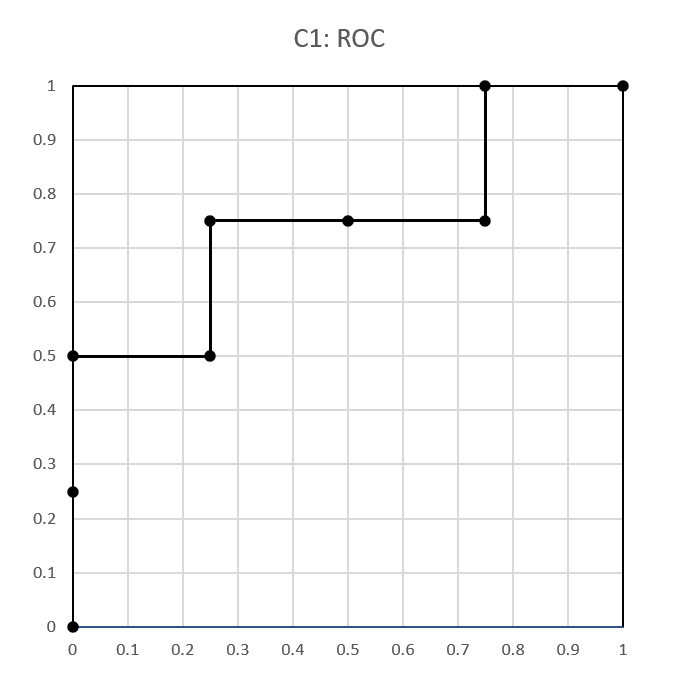
\includegraphics[width=6cm,height=6cm]{c1-roc.PNG}
		\caption{$C_1\;$ROC曲线}
	\end{figure}
	
	AUC
	$=\frac{1}{2}\sum_1^8(x_{i+1}-x_i)(y_i+y_{i+1})
	=0.75$\\

	$C_2$:
	\begin{figure}[H]
		\centering
		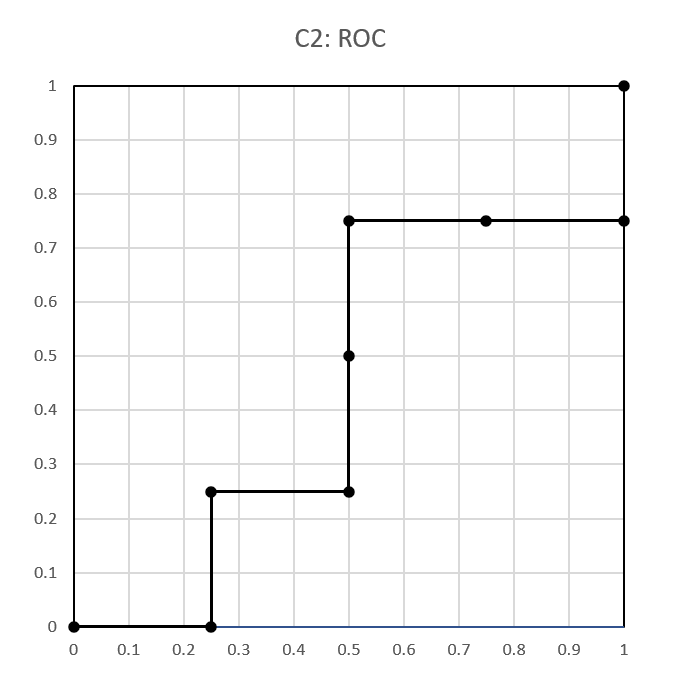
\includegraphics[width=6cm,height=6cm]{c2-roc.PNG}
		\caption{$C_2\;$ROC曲线}
	\end{figure}

	AUC
	$=\frac{1}{2}\sum_1^8(x_{i+1}-x_i)(y_i+y_{i+1})
	=0.4375$


	(2) 
	$C_1$:
	\begin{figure}[H]
		\centering
		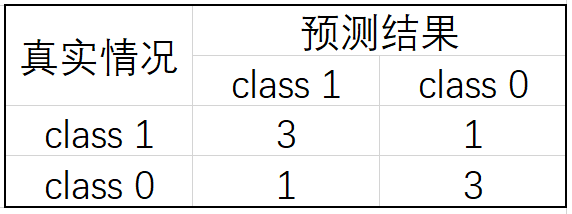
\includegraphics[width=5.7cm,height=2.1cm]{c1-cm.PNG}
		\caption{$C_1$混淆矩阵}
	\end{figure}

	$P=\frac{TP}{TP+FP}=0.75$

	$R=\frac{TP}{TP+FN}=0.75$

	$F_1=\frac{2*P*R}{P+R}=0.75$\\

	$C_2$:
	\begin{figure}[H]
		\centering
		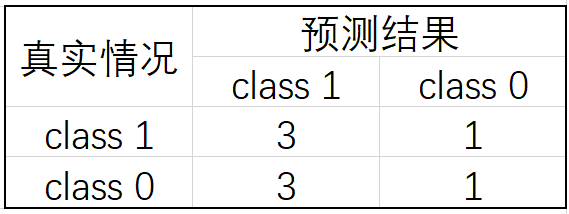
\includegraphics[width=5.7cm,height=2.1cm]{c2-cm.PNG}
		\caption{$C_2$混淆矩阵}
	\end{figure}

	$P=\frac{TP}{TP+FP}=0.5$

	$R=\frac{TP}{TP+FN}=0.75$

	$F_1=\frac{2*P*R}{P+R}=0.6$
	\end{spacing}

	
\end{document}